%%%%%%%%%%%%%%%%%%%%%%%%%%%%%%%%%%%%%%%%%%%%%%%%%%%%%%%%%%%%%%%%%%%%%%
%% Copyright (c) 2016 Carsten Wulff Software, Norway
%% %%%%%%%%%%%%%%%%%%%%%%%%%%%%%%%%%%%%%%%%%%%%%%%%%%%%%%%%%%%%%%%%%%%
%% Created       : wulff at 2016-11-5
%% %%%%%%%%%%%%%%%%%%%%%%%%%%%%%%%%%%%%%%%%%%%%%%%%%%%%%%%%%%%%%%%%%%%
%% This program is free software: you can redistribute it and/or modify
%% it under the terms of the GNU General Public License as published by
%% the Free Software Foundation, either version 3 of the License, or
%% (at your option) any later version.
%%
%% This program is distributed in the hope that it will be useful,
%% but WITHOUT ANY WARRANTY; without even the implied warranty of
%% MERCHANTABILITY or FITNESS FOR A PARTICULAR PURPOSE.  See the
%% GNU General Public License for more details.
%%
%% You should have received a copy of the GNU General Public License
%% along with this program.  If not, see <http://www.gnu.org/licenses/>.
%%%%%%%%%%%%%%%%%%%%%%%%%%%%%%%%%%%%%%%%%%%%%%%%%%%%%%%%%%%%%%%%%%%%%%
%\documentclass[final,11pt]{IEEEtran}
\documentclass[crop,border=0pt]{standalone}
\usepackage{times}


%\usepackage{placeins}
\usepackage{upgreek}
\usepackage{amssymb,amsmath}
\usepackage{cite}
\usepackage{verbatim}
\usepackage{listings}
\usepackage{xcolor}
\usepackage{flafter}
\usepackage{booktabs}
\usepackage{url}
\usepackage{ textcomp }

\hyphenation{op-tical net-works semi-conduc-tor}


% -JSON styel

%\definecolor{darkGreen}{rgb}{0,0.2097,0}
%\newcommand{\myfigwidth}{\linewidth}
%\newcommand{\myfigwidtha}{\linewidth}
%\newcommand{\myfigwidthl}{\textwidth}
%\newcommand{\myfigwidthc}{0.6\linewidth}


\newcommand{\myfigwidtha}{3.3in}
\newcommand{\myfigwidthl}{7in}
\newcommand{\myfigwidthc}{2in}
%\newcommand{\myfigwidthe}{3.2in}
%\newcommand{\myfigwidthb}{5in}

\newcommand{\myfigname}{fig_}
\newcommand{\reg}[2]{{\figurename} \ref{#1}(#2)}
\newcommand{\req}[1]{{\figurename} \ref{#1}}
%\newcommand{\myeqname}{eq:}
%\newcommand{\req}[1]{(\ref{\myeqname#1})}

\definecolor{armygreen}{rgb}{0, 0.5, 0}
\newcommand{\missing}[1]{{ #1}}
\newcommand{\edit}[1]{{ #1}}
\newcommand{\secedit}[1]{{ #1}}
\newcommand{\deleted}[1]{{ #1}}
\newcommand{\moved}[1]{{ #1}}

%\newcommand{\missing}[1]{{\color{red} #1}}
%\newcommand{\edit}[1]{{\color{red} #1}}
%\newcommand{\secedit}[1]{{\color{armygreen} #1}}
%\newcommand{\deleted}[1]{{\color{violet} #1}}
%\newcommand{\moved}[1]{{\color{blue} #1}}

\newcommand{\SD}{Sigma-Delta }
\newcommand{\eqn}[1]{
  \begin{math}
    #1
  \end{math}}

\newcommand\JSONnumbervaluestyle{\color{blue}}
\newcommand\JSONstringvaluestyle{\color{red}}



\newif\ifcolonfoundonthisline

\makeatletter

\lstdefinestyle{json}
{
  showstringspaces    = false,
  keywords            = {false,true},
  alsoletter          = 0123456789.,
  morestring          = [s]{"}{"},
  stringstyle         = \ifcolonfoundonthisline\JSONstringvaluestyle\fi,
  MoreSelectCharTable =%
  \lst@DefSaveDef{`:}\colon@json{\processColon@json},
  basicstyle          = \fontsize{7}{7}\ttfamily,
  keywordstyle        = \fontsize{7}{7}\ttfamily\bfseries,
}

% flip the switch if a colon is found in Pmode
\newcommand\processColon@json{%
  \colon@json%
  \ifnum\lst@mode=\lst@Pmode%
  \global\colonfoundonthislinetrue%
  \fi
}

\lst@AddToHook{Output}{%
  \ifcolonfoundonthisline%
  \ifnum\lst@mode=\lst@Pmode%
  \def\lst@thestyle{\JSONnumbervaluestyle}%
  \fi
  \fi
  % override by keyword style if a keyword is detected!
  \lsthk@DetectKeywords%
}

% reset the switch at the end of line
\lst@AddToHook{EOL}%
{\global\colonfoundonthislinefalse}

\makeatother

% \lstset{  basicstyle=\tiny}

% \lstset{
% basicstyle=\fontsize{11}{13}\selectfont\ttfamily
% }


\lstset{language=Java}




%\usepackage[paperwidth=\maxdimen,paperheight=\maxdimen]{geometry}


\usepackage{tikz,pgfplots}
\usepackage{ifthen}
\usepackage{calc}
\usetikzlibrary{patterns}
%\usepackage[tightpage,active]{preview}
\usetikzlibrary{circuits.logic.US}
\usetikzlibrary{circuits.ee.IEC}
\usepgflibrary{shapes.arrows}
\usepgflibrary{arrows}
\usepackage{circuitikz}


% circuitikz draws bipole outlines (resistors, diodes, capacitors) at
% bipoles/thickness times the ambient line width, and the default is 2.
% That makes a circuitikz resistor visibly heavier than the wire it sits
% on, and heavier than the hand rolled zig-zag in ckt_lib.tex. One is the
% house width: everything is drawn at the environment's own thickness.
% Arrow tips: one filled tip everywhere, set through the '>' knob so a
% figure only ever writes ->, <- or <->. Latex (from arrows.meta)
% scales with the line width, so it stays in proportion if a drawing
% is ever set thicker or thinner than the house 'thick'.
\usetikzlibrary{arrows.meta}
\tikzset{>={Latex}}

\ctikzset{bipoles/thickness=1}
\ctikzset{tripoles/mos style/arrows}
\ctikzset{tripoles/pmos style/emptycircle}
%\PreviewEnvironment{circuitikz}
\pagestyle{empty}


\tikzstyle{cicfill}=[minimum size=1.4em]
\tikzstyle{stuff_fill}=[rectangle,fill=white,minimum size=1.4em]

\newcommand{\grayOne}{0.3 }
\newcommand{\grayTwo}{0.15 }
\newcommand{\grayThree}{0.26 }
\newcommand{\grayFour}{0.41 }
\newcommand{\grayFive}{0.61 }
\newcommand{\graySix}{0.85 }

%- Gray tone
%\definecolor{active}{rgb}{\graySix,\graySix,\graySix}
%\definecolor{poly}{rgb}{\grayFive,\grayFive,\grayFive}
%\definecolor{contact}{rgb}{\graySix,\graySix,\graySix}
%\definecolor{mOne}{rgb}{\grayFour,\grayFour,\grayFour}
%\definecolor{mTwo}{rgb}{\graySix,\graySix,\graySix}
%\definecolor{mThree}{rgb}{\grayThree,\grayThree,\grayThree}
%\definecolor{mFour}{rgb}{\grayTwo,\grayTwo,\grayTwo}

\definecolor{grey}{rgb}{1,1,1}
\definecolor{lightgrey}{rgb}{\grayFour,\grayFour,\grayFour}
\definecolor{active}{rgb}{0.4,1,0.6}
\definecolor{poly}{rgb}{1.0,0.5,0.5}
\definecolor{cut}{rgb}{0.91,0.91,0}
\definecolor{mOne}{rgb}{0.36,0.36,1}
\definecolor{mTwo}{rgb}{0.655,0.655,0}
\definecolor{mThree}{rgb}{0.3,1,1}
\definecolor{mFour}{rgb}{0,0.2097,0}
\begin{document}


% The nRF5340 as a block diagram, simplified from the product
% specification. The application core (Arm Cortex-M33 at 128 MHz, 1 MB
% flash, 512 kB RAM) and the network core (Cortex-M33 at 64 MHz, 256 kB
% flash, 64 kB RAM) each carry a grid of peripherals, and the two cores
% talk through IPC. The point of the figure is the size of the RADIO
% box, drawn in red: the entire 2.4 GHz transceiver, the subject of the
% whole chapter, is one block among some fifty. Bus bridges and the
% debug subsystem of the original are left out. Redrawn so the book does
% not carry the datasheet figure.

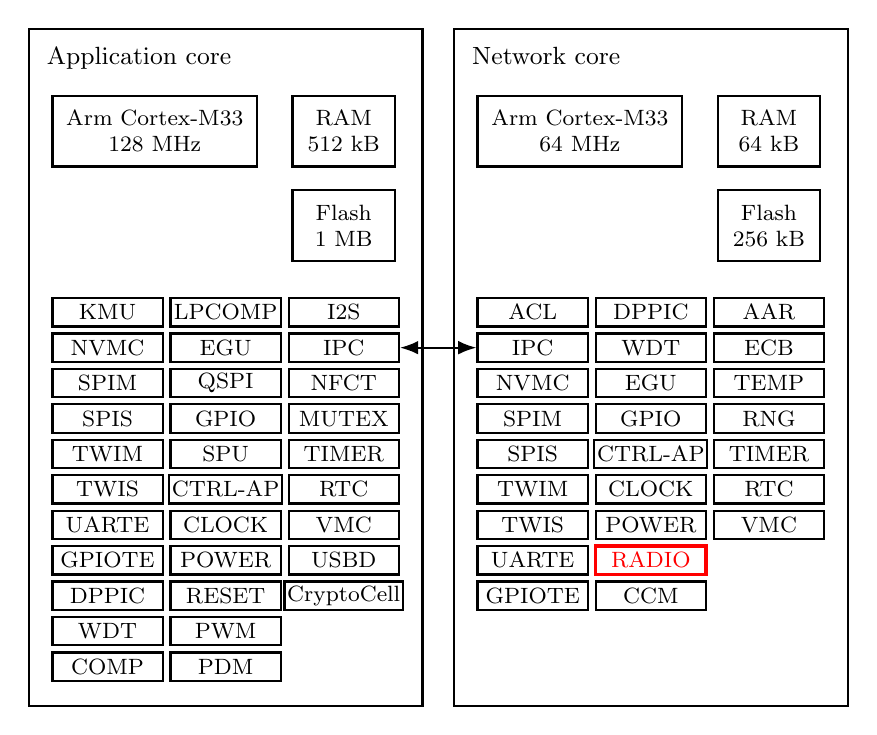
\begin{tikzpicture}[thick, font=\footnotesize]

  \tikzset{per/.style={draw, fill=white, minimum width=1.4cm,
                       minimum height=0.36cm, inner sep=1pt},
           mem/.style={draw, minimum height=0.9cm, align=center}}

  % application core
  \draw (0,0) rectangle (5.0,8.6);
  \node[anchor=north west, font=\small] at (0.1,8.5) {Application core};
  \node[mem, minimum width=2.6cm] at (1.6,7.3) {Arm Cortex-M33\\128 MHz};
  \node[mem, minimum width=1.3cm] at (4.0,7.3) {RAM\\512 kB};
  \node[mem, minimum width=1.3cm] at (4.0,6.1) {Flash\\1 MB};
  \foreach \n [count=\i from 0] in {KMU, NVMC, SPIM, SPIS, TWIM, TWIS,
      UARTE, GPIOTE, DPPIC, WDT, COMP, LPCOMP, EGU, QSPI, GPIO, SPU,
      CTRL-AP, CLOCK, POWER, RESET, PWM, PDM, I2S, IPC, NFCT, MUTEX,
      TIMER, RTC, VMC, USBD, CryptoCell} {
    \pgfmathtruncatemacro{\c}{int(\i/11)}
    \pgfmathtruncatemacro{\r}{mod(\i,11)}
    \node[per] (a\i) at (1.0+1.5*\c, 5.0-0.45*\r) {\n};
  }

  % network core
  \draw (5.4,0) rectangle (10.4,8.6);
  \node[anchor=north west, font=\small] at (5.5,8.5) {Network core};
  \node[mem, minimum width=2.6cm] at (7.0,7.3) {Arm Cortex-M33\\64 MHz};
  \node[mem, minimum width=1.3cm] at (9.4,7.3) {RAM\\64 kB};
  \node[mem, minimum width=1.3cm] at (9.4,6.1) {Flash\\256 kB};
  \foreach \n [count=\i from 0] in {ACL, IPC, NVMC, SPIM, SPIS, TWIM, TWIS,
      UARTE, GPIOTE, DPPIC, WDT, EGU, GPIO, CTRL-AP, CLOCK, POWER,
      RADIO, CCM, AAR, ECB, TEMP, RNG, TIMER, RTC, VMC} {
    \pgfmathtruncatemacro{\c}{int(\i/9)}
    \pgfmathtruncatemacro{\r}{mod(\i,9)}
    \node[per] (n\i) at (6.4+1.5*\c, 5.0-0.45*\r) {\n};
  }
  \node[per, draw=red, very thick, text=red] at (n16) {RADIO};

  % the cores share data through IPC
  \draw[<->] (a23.east) -- (n1.west);

\end{tikzpicture}
\end{document}
